\documentclass[a4paper]{scrartcl}
\usepackage{amsmath}
\usepackage{mathtools}
\usepackage{titlesec}
\usepackage[utf8]{inputenc}
\usepackage[polish]{babel}
\usepackage{textcomp}
\usepackage[T1]{fontenc}
\usepackage{amsthm}
\usepackage{amsfonts}

\title{Sieci komputerowe - warsztaty 4}
\author{Dawid Żywczak}
\date{21 kwietnia 2020}

\begin{document}
\maketitle
\qquad Jako dowód wykonania zadania przesyłam zrzuty ekranu, tak jak ostatnio oraz postaram się odpowiedzieć na zadane pytania.\\
\begin{figure}
  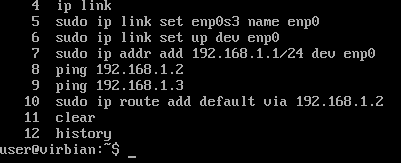
\includegraphics[width=\linewidth]{hist_1.png}
  \caption{Historia terminala na maszynie Virbian1}
\end{figure}
\begin{figure}
  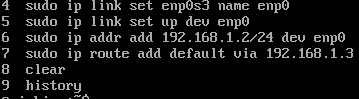
\includegraphics[width=\linewidth]{hist_2.png}
  \caption{Historia terminala na maszynie Virbian2}
\end{figure}
\begin{figure}
  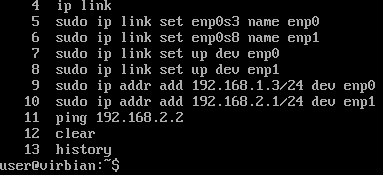
\includegraphics[width=\linewidth]{hist_3.png}
  \caption{Historia terminala na maszynie Virbian3}
\end{figure}
\begin{figure}
  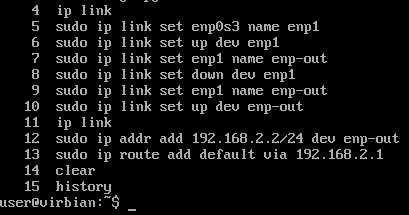
\includegraphics[width=\linewidth]{hist_4.png}
  \caption{Historia terminala na maszynie Virbian4}
\end{figure}
\begin{figure}
  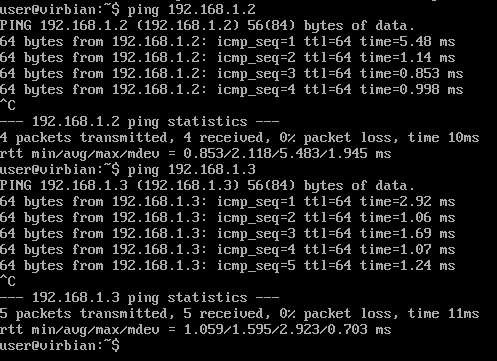
\includegraphics[width=\linewidth]{pings_connected.png}
  \caption{Sprawdzenie osiągalności maszyn w local0}
\end{figure}
\begin{figure}
  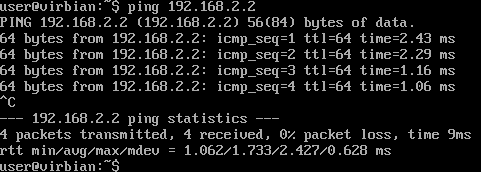
\includegraphics[width=\linewidth]{ping_connected1.png}
  \caption{Sprawdzenie osiągalności maszyn w local1}
\end{figure}
\begin{figure}
  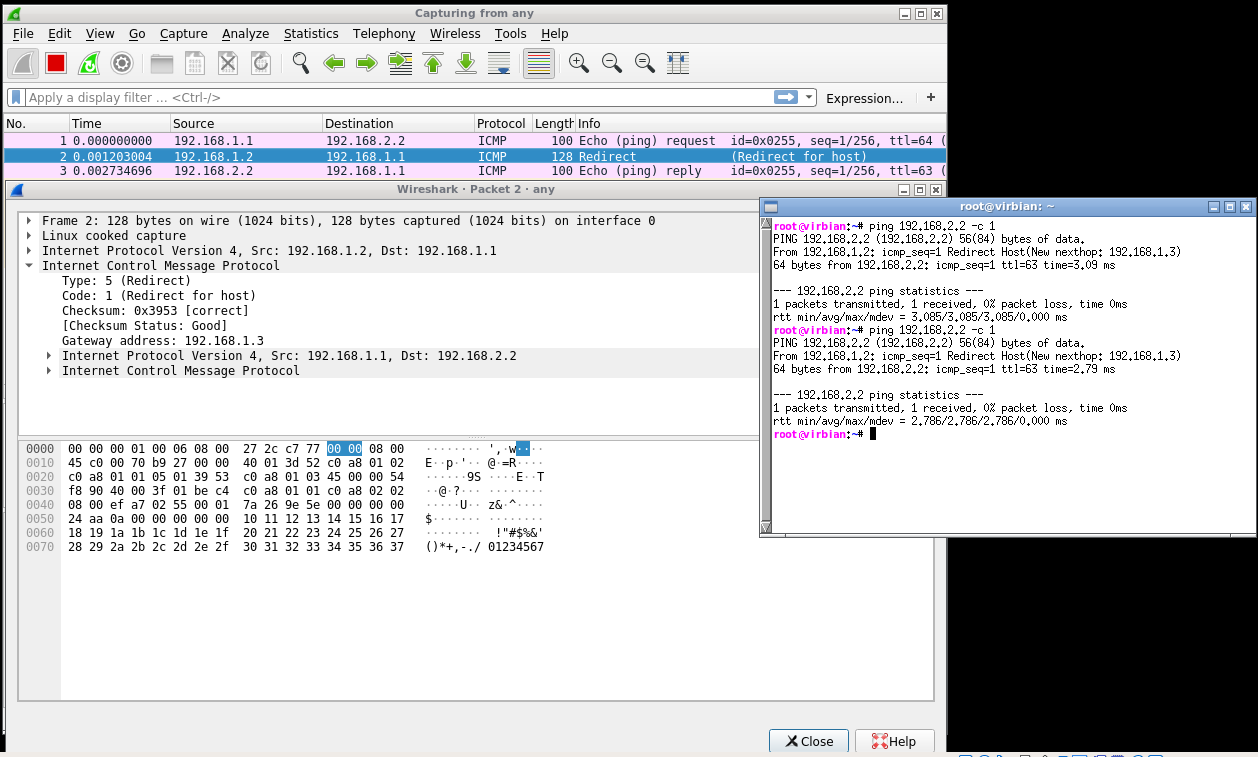
\includegraphics[width=\linewidth]{redirect_vib1.png}
  \caption{Sprawdzenie osiągalności maszyn w local1}
\end{figure}
Odpowiadając na pytania. Maszyna Virbian2 sugeruje bezpośrednie przesyłanie pakietów do maszyny Virbian3. Taka zmiana ma sens, ponieważ ''oszczędzamy'' jeden skok pakietu. Według mnie maszyna Virbian2 mogła wykryć ten problem w trakcie aktualizowania swojej tablicy routingu, ponieważ wie, że jest bezpośrednio połączona ze wszystkimi komputerami w sieci local0, zatem nie ma sensu kierować przez nią ruchu, gdy można wysłać pakiet bezpośrednio.
\end{document}